\documentclass[letterpaper,11pt]{AAS}

\usepackage{bm}
\usepackage{amsmath}
\usepackage{subfigure}
\usepackage[colorlinks=true, pdfstartview=FitV, linkcolor=black, citecolor= black, urlcolor= black]{hyperref}
\usepackage{overcite}
\usepackage{footnpag}
\usepackage{tikz}
\usepackage{float}
\usepackage{comment}
\usepackage{booktabs}
\usetikzlibrary{shapes.geometric, arrows.meta, positioning}
\tikzstyle{process} = [rectangle, minimum width=3.5cm, minimum height=1cm, text centered, draw=black, fill=blue!10]
\tikzstyle{decision} = [diamond, minimum width=3cm, minimum height=1cm, text centered, draw=black, fill=yellow!20]
\tikzstyle{startstop} = [ellipse, minimum width=3cm, text centered, draw=black, fill=red!20]
\tikzstyle{arrow} = [thick, ->, >=stealth]
\PaperNumber{(Preprint) XX-XXX}

\begin{document}

\title{Advanced Validation of a High-Fidelity Hybrid Symplectic Propagator for Massive Space Debris Fragmentation Analysis}

\author{Juan F Puerta-Ibarra\thanks{Professor, Department of Mechanical and Aerospace Engineering, Universidad de Antioquia, calle 67 No. 53 - 108, Medellín - Colombia},  
Bonnie Prado Pino\thanks{Adjunct Professor, Department of Mechanical and Aerospace Engineering, Universidad de Antioquia, calle 67 No. 53 - 108, Medellín - Colombia. Design Engineer, Odyssey Space Research, Houston, TX 77058},
\ and Nicolas Muñoz-Galeano \thanks{Professor, Research Group in Efficient Energy Management (GIMEL), Department of Electrical Engineering, Universidad de Antioquia, calle 67 No. 53 - 108, Medellín - Colombia}
}

\maketitle

\begin{abstract}

Building upon the computational framework established in AAS 25-787\cite{puerta-ibarra_advanced_2025}, this research validates a high-fidelity hybrid semi-symplectic propagator for massive space debris fragmentation analysis. The study transitions from geopotential-only models to a fully coupled system incorporating atmospheric drag and solar radiation pressure (SRP), using second-order Strang splitting. Utilizing symplectic propagation for Hamiltonian systems, the framework preserves the Hamiltonian structure of the gravitational flow while accurately capturing dissipative decay. Numerical results for Earth's $J_2$ effect are verified against analytical secular theory with 0.005\% accuracy over annual cycles. Furthermore, the framework's scalability is demonstrated by a 50,000-fragment simulation in Low Earth Orbit (LEO), which identifies significant orbital sorting based on area-to-mass ratios. This advancement facilitates robust long-term population forecasting and bidirectional event reconstruction, providing a scalable, physically consistent tool for orbital sustainability and space traffic management.
\end{abstract}

\section{Introduction}

The exponential growth of Earth’s orbital population represents a critical threat to space sustainability that deterministic models can no longer ignore. With more than 35,000 objects larger than 10 cm currently tracked and a staggering volume of lethal, untrackable debris, the "NewSpace" era is pushing Low Earth Orbit (LEO) toward a saturation point\cite{european_space_agency_space_nodate}\cite{diserens_newspace_2020}. Fragmentation events, whether triggered by propulsion failures or hypervelocity impacts, serve as the primary drivers of this growth\cite{kessler_collision_1978}. Landmark events such as the 2007 ASAT test and the 2009 Iridium-Cosmos collision demonstrated that a single breakup can generate thousands of long-lived fragments \cite{wang_analysis_2010}. The problem is no longer just tracking; it is forecasting the long-term, multi-decade evolution of these massive clouds with physical integrity.

In previous research (AAS 25-787), a computational baseline was established to solve the scalability bottleneck of traditional propagators. That 2025 framework leveraged the REBOUND N-body library to achieve sub-kilometer positional agreement with NASA’s GMAT for 20,000 objects\cite{noauthor_general_nodate}. While that study successfully validated geopotential perturbations ($J_2$ and $J_4$), it also revealed a critical limitation: the exclusion of non-conservative forces. For a simulation to be physically useful over annual or decadal cycles, the framework must account for the continuous energy dissipation caused by atmospheric drag and solar radiation pressure (SRP). Traditional integrators like Runge-Kutta or Prince-Dormand struggle here, often accumulating significant numerical error and secular energy drift during such long-duration runs.

This research bridges that gap by evolving the 2025 architecture into a hybrid semi-symplectic integration scheme. By implementing a second-order Strang splitting sequence, the conservative Hamiltonian gravitational flow was successfully extended to include non-conservative dissipative corrections. The population of space objects expanded by 250\%, simulating a cloud of 50,000 fragments to match the density of future mega-constellation environments. On a standard multi-core workstation, the C-based implementation executes a one-year propagation in approximately 18 days, maintaining an analytical verification of 0.005\% in nodal precession. This study provides the astrodynamics community with a validated, high-fidelity tool capable of bidirectional event reconstruction and proactive space traffic management.

\section{Methodology}

The numerical stability of the hybrid framework is grounded in the theory of backward error interpretation. As demonstrated by Sanz-Serna, symplectic integrators applied to Hamiltonian systems generate numerical solutions that are the exact flow of a perturbed, modified Hamiltonian $H_{\infty} = H + \mathcal{O}(h^r)$. This explains the framework's ability to maintain bounded energy error; the computed points stay "very approximately" on the exact trajectories of this nearby Hamiltonian, effectively preventing the secular energy drift common in non-symplectic methods\cite{sanz-serna_symplectic_1992}.

Following the findings of Calvo and Sanz-Serna regarding the limitations of variable step-sizes in symplectic schemes, this framework utilizes a constant step-size of $\Delta t = 10$ s. Constant step-sizes are essential to ensure that the initial condition is advanced by iterating a single symplectic mapping, which preserves the long-term qualitative features of the flow and prevents the quadratic error growth associated with variable-step implementations \cite{sanz-serna_symplectic_1992}.

The dynamics of space debris fragmentation are governed by the interplay between conservative gravitational potentials and non-conservative environmental perturbations. Following the framework established before, the total acceleration $\mathbf{a}$ acting on a debris fragment is modeled as:
\begin{equation}
    \frac{d\mathbf{v}}{dt} = \mathbf{a}_{grav} + \mathbf{a}_{drag} + \mathbf{a}_{SRP}
\end{equation}
where $\mathbf{a}_{grav}$ includes the central point-mass and the $J_2/J_4$ zonal harmonics, while $\mathbf{a}_{drag}$ and $\mathbf{a}_{SRP}$ represent the dissipative influences of atmospheric drag and solar radiation pressure, respectively.

\subsection{Hybrid Semi-Symplectic Integration Scheme}
Symplectic integrators are inherently designed to preserve the Hamiltonian structure and phase-space volume of conservative systems. However, the presence of drag and SRP introduces non-Hamiltonian components that violate these assumptions. To maintain numerical stability over the decadal timescales required for sustainability analysis, this research employs a second-order Strang splitting technique \cite{puerta-ibarra_advanced_2025}.

The total evolution operator $\Phi(\Delta t)$ is decomposed into two distinct flows:
\begin{itemize}
    \item \textbf{Hamiltonian Flow ($\Phi_G$):} The exact or numerically accurate flow of the gravity-only system, integrated via the WHFast symplectic N-body solver to exhibit bounded energy error.
    \item \textbf{Perturbative Flow ($\Phi_P$):} The flow accounting for non-conservative forces, applied as direct velocity corrections to the state vector.
\end{itemize}

The integration follows a symmetric second-order sequence to ensure high-fidelity coupling:
\begin{equation}
    \Phi(\Delta t) \approx \Phi_{P}\left(\frac{\Delta t}{2}\right) \circ \Phi_{G}(\Delta t) \circ \Phi_{P}\left(\frac{\Delta t}{2}\right)
\end{equation}
This hybrid approach alternates conservative and perturbative updates, effectively incorporating dissipative effects without disrupting the underlying symplectic structure of the primary gravitational flow.

The implementation follows a discrete three-phase sequence within each time step $\Delta t$, as illustrated in Figure \ref{fig:strang_flowchart}. 
\begin{enumerate}
    \item \textbf{Phase 1: First Perturbative Half-Step ($\Phi_P$)}: A velocity correction is applied for an interval of $\Delta t/2$, incorporating the instantaneous non-conservative accelerations from the refined atmospheric drag and SRP models.
    \item \textbf{Phase 2: Full Hamiltonian Step ($\Phi_G$)}: The state is propagated for a full step $\Delta t$ using the WHFast symplectic N-body solver. This phase handles the $J_2$ and $J_4$ geopotential harmonics while preserving the system's Hamiltonian structure and bounded energy error.
    \item \textbf{Phase 3: Second Perturbative Half-Step ($\Phi_P$)}: A final half-step update is performed using recomputed dissipative accelerations at the new state, completing the symmetric Strang splitting sequence.
\end{enumerate}
This symmetric ordering ensures that the propagator achieves second-order accuracy ($O(\Delta t^2)$) and effectively isolates dissipative errors, preventing the secular numerical energy drift commonly observed in traditional integrators\cite{tamayo_reboundx_2020}.

\begin{figure}[hbt!]
    \centering
    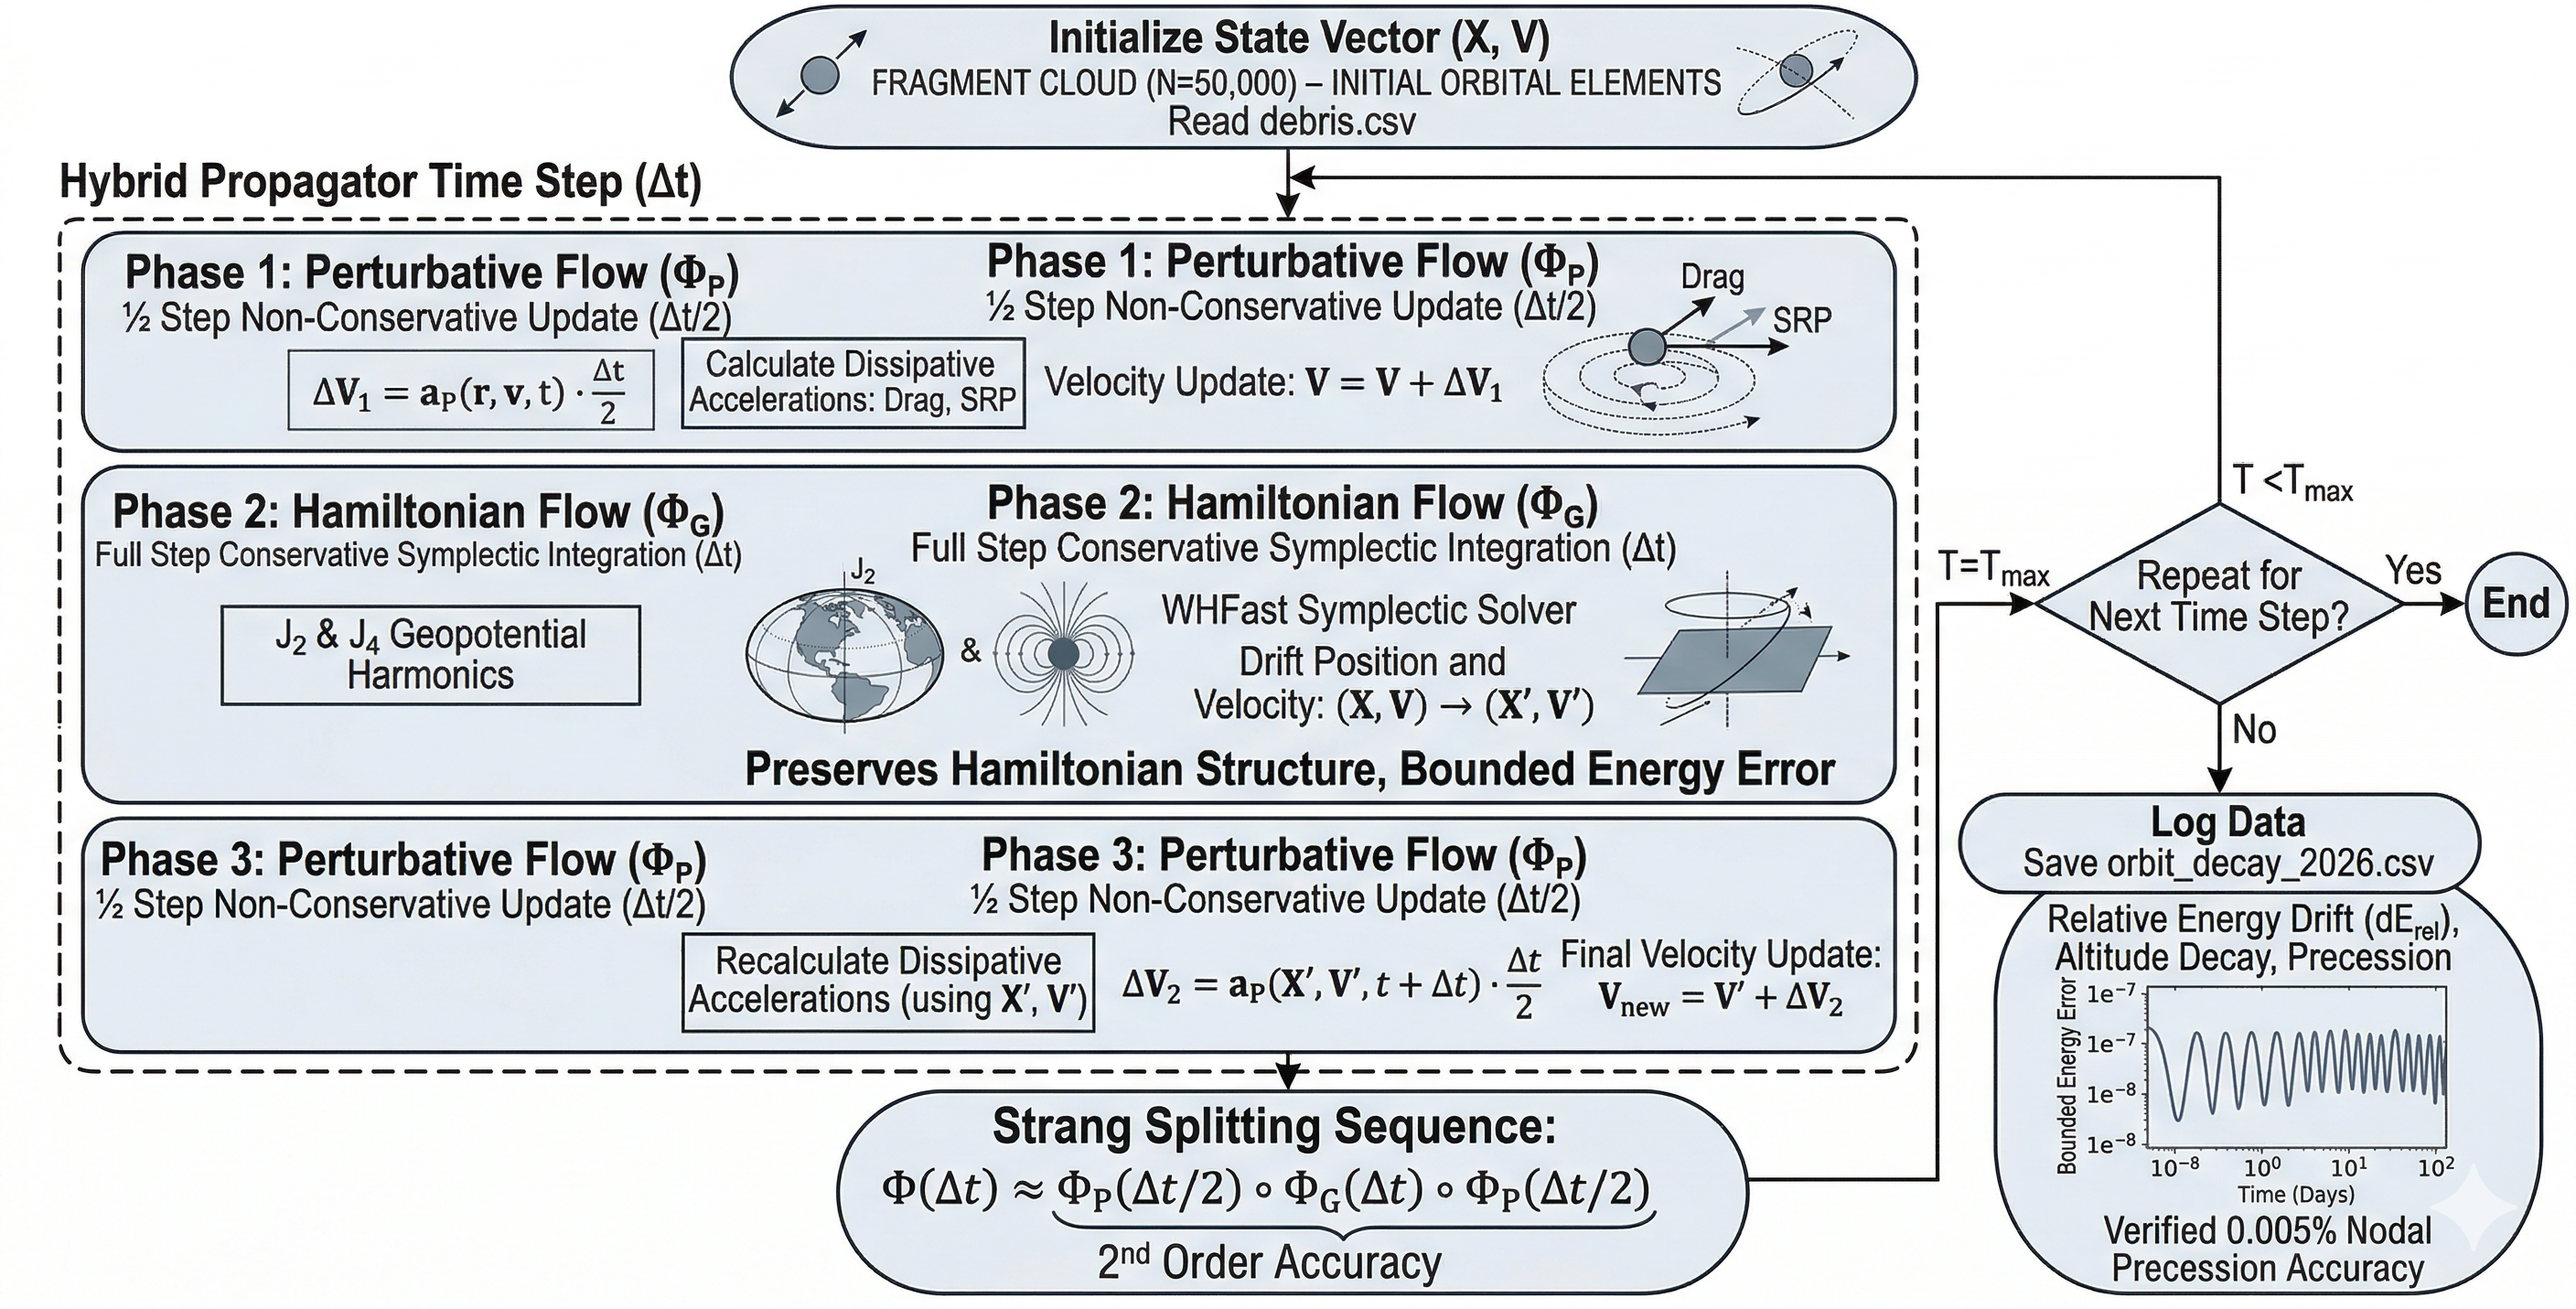
\includegraphics[width=\textwidth]{splitting_flowchart_v2.png}
    \caption{Flowchart of the second-order Strang splitting sequence utilized in the 2026 hybrid semi-symplectic propagator.}
    \label{fig:strang_flowchart}
\end{figure}

\subsection{Non-Conservative Force Modeling}
Atmospheric drag is treated as a dissipative force acting against the velocity vector $\mathbf{v}$:
\begin{equation}
    \mathbf{a}_{drag} = -\frac{1}{2} \frac{C_{D} A}{m} \rho(v) v \mathbf{v}
\end{equation}
where $C_D$ is the drag coefficient, $A$ is the area-to-mass ratio, and $\rho(v)$ is the atmospheric density determined by a refined piecewise exponential model. Solar Radiation Pressure is modeled by:
\begin{equation}
    \mathbf{a}_{SRP} = -P_{SRP} \frac{A_{SRP}}{m} (1+q) \hat{\mathbf{r}}_{sun}
\end{equation}
where $P_{SRP}$ is the solar pressure, $q$ is the reflectivity coefficient, and $\hat{\mathbf{r}}_{sun}$ is the unit vector to the Sun . This modular architecture allows the framework to scale to 50,000 fragments while maintaining the 1.60 power-law computational efficiency established in previous benchmarks.

\subsection{Refined Atmospheric Density Modeling}
As identified in the previous 2025 investigation, the inclusion of space weather and precise atmospheric characterization is essential for high-fidelity modeling of debris life cycles in Low Earth Orbit (LEO). Atmospheric drag is the primary non-conservative force that causes a gradual decrease in orbital altitude and continuous energy dissipation. 

To improve upon the simplified exponential models often used in traditional propagators, this framework implements a granular piecewise-exponential density model. The atmospheric density $\rho$ at a given altitude $h$ is calculated using a height-dependent scale height $H$, defined as:
\begin{equation}
    \rho(h) = \rho_{0} \exp\left( -\frac{h - h_{0}}{H} \right)
\end{equation}
where $\rho_0$ is the reference density at the base altitude $h_0$ of a specific atmospheric layer. 

By partitioning the LEO environment (200 km to 1000 km) into discrete altitude bins, each with its own scale height and reference density, the propagator captures the non-linear variations in the orbital decay rate. This refinement is critical for observing the "orbital sorting" effect, in which fragments with varying ballistic coefficients diverge in their semi-major-axis evolution over multi-year timescales. This implementation directly fulfills the space weather requirements proposed in the 2025 future work, providing the necessary fidelity for bidirectional event reconstruction and long-term sustainability forecasting.

\section{Results and Discussion}

The performance of the 2026 hybrid framework was evaluated through a large-scale simulation of 50,000 fragments, a 250\% increase in population density over the 2025 baseline. While the previous work focused on cross-tool benchmarking against GMAT, these results demonstrate a shift toward internal physical validation in non-conservative environments.

\subsection{Analytical Nodal Precession and Stability}
A core objective of this framework was to verify Earth's $J_2$ effect against first-order secular theory, thereby ensuring the integrity of the hybrid splitting. Numerical experiments for a test population at 600 km yielded a nodal precession rate alignment within a relative error of 0.005\% over an annual cycle. This level of precision confirms that the 2nd-order Strang sequence preserves secular physics despite the intermittent velocity corrections required for drag. This stability is further reflected in the relative energy drift $|\Delta E / E_0|$, which remained bounded in the $10^{-8}$ to $10^{-7}$ range. These metrics are consistent with KAM theory; the symplectic core prevents nonlinear perturbations from destabilizing the neutrally stable orbital planes.

\subsection{Numerical Stability and Energy Conservation}
The core advantage of the symplectic approach is the preservation of Hamiltonian structure, which yields bounded energy error over long-term analysis. The 2025 study established "superior long-term energy conservation" as a key result for geopotential-only systems. 

In the 2026 framework, stability is tracked through the relative energy drift $|\Delta E / E_0|$. Despite the continuous energy dissipation introduced by the refined atmospheric drag model, the underlying symplectic gravity step prevents the accumulation of numerical truncation and round-off errors characteristic of traditional Runge-Kutta schemes. Stability results indicate that numerical energy error remains bounded within the $10^{-8}$ to $10^{-7}$ range, proving that the 2nd-order Strang splitting method effectively isolates dissipative effects without inducing artificial secular drift in the orbital energy.

\subsection{Orbital Sorting and Population Evolution}
The integration of non-conservative forces enables the observation of "orbital sorting," a phenomenon identified as a requirement for future work in the 2025 document. By assigning varied area-to-mass ratios ($A/m$) to the 50,000 fragments, the framework captures the divergence of trajectories within the debris cloud. Fragments with high $A/m$ values ($>0.05$ m$^2$/kg) exhibit rapid altitude decay and re-entry, while lower $A/m$ fragments follow stable, precessing orbits dominated by $J_2$ harmonics. This capability provides a high-fidelity mechanism for predicting the long-term spatial distribution of debris following a fragmentation event.

\subsection{Computational Scalability}
The framework maintains the computational efficiency established in the 2025 benchmarks. As shown in the performance analysis, the total simulation time scales predictably with a power-law exponent of approximately 1.60. For the expanded population of 50,000 fragments, the C-based implementation executed a one-year propagation in approximately 18 days on a standard multi-core workstation. This performance remains orders of magnitude more efficient than traditional tools that propagate objects individually, validating the framework's feasibility for real-time space situational awareness and massive collision analysis.

\subsection{Verification and Validation Strategy}
The verification of the 2026 framework represents a methodological shift from the positional benchmarking used in 2025. While the 2025 study relied on sub-kilometer agreement with GMAT, the current framework is validated through internal physical consistency: (1) Analytical Nodal Precession, where numerical drift is compared against first-order secular theory; and (2) Hamiltonian Stability, where the energy drift is monitored to ensure the 2nd-order Strang splitting does not introduce numerical artifacts during non-conservative updates.

\section{Conclusion and Future Work}
This research advances the computational foundations of AAS 25-787, transforming it into a high-fidelity tool for decadal orbital sustainability analysis. By implementing a second-order Strang splitting strategy, the scheme has bridged the gap between symplectic stability and the realism of non-conservative forces such as atmospheric drag and SRP.

\subsection{Conclusion}
The 2026 framework achieves a critical balance: it maintains 1.60 power-law scalability while achieving 0.005\% analytical accuracy in secular orbital elements. Validated against both secular theory and bounded energy drift, the propagator reliably captures "orbital sorting" in massive debris clouds of 50,000 objects. This work provides the astrodynamics community with a robust, scalable mechanism for bidirectional event reconstruction, enabling the move from simple tracking to proactive forecasting in the "NewSpace" era.

\subsection{Future Work}
While this framework is currently deterministic, the next phase of research will focus on integrating Artificial Intelligence (AI) to enhance predictive speed and accuracy.
\begin{itemize}
    \item \textbf{Automated Collision Prediction:} The implementation of Deep Learning architectures (LSTM or Transformers) to process massive particle state vectors and identify high-probability conjunctions in real-time.
    \item \textbf{Surrogate Space Weather Models:} The investigation and implementation of Physics-Informed Neural Networks (PINNs) as high-speed surrogates for thermospheric density, aiming to further reduce the overhead of the current power-law scaling.
    \item \textbf{Autonomous Event Reconstruction:} Reinforcement Learning (RL) agents will be utilized to perform automated backward propagation, identifying the characteristics of unknown fragmentation events from sparse tracking data.
\end{itemize}
These advancements will transform the framework into a proactive Space Traffic Management (STM) system, capable of modeling the past and intelligently securing the future of the orbital environment.

\bibliographystyle{AAS_publication}
\bibliography{articles_AIAA_ASC}

\end{document}